\documentclass{amsart}
\usepackage{graphicx}
\usepackage[margin=3cm]{geometry}

% Para bibliografía
\usepackage[spanish]{babel}
\usepackage[babel]{csquotes}
\usepackage[backend=biber, style=apa]{biblatex}
\DeclareLanguageMapping{spanish}{spanish-apa}
\bibliography{sources/references.bib}

% Estilos de URL
\usepackage{hyperref}
\hypersetup{
    colorlinks=true,
    linkcolor=magenta,
    filecolor=magenta,      
    urlcolor=cyan,
    pdftitle={Overleaf Example},
    pdfpagemode=FullScreen,
    }
\urlstyle{same}

% Para figuras
\usepackage{subfig}
% Para tablas
\usepackage{booktabs}


\begin{document}

% ---------------------------------- Portada ----------------------------------
    \begin{center}
        {\bfseries\LARGE Instituto Tecnológico de Monterrey\par}
        %\vspace{0.5cm}
        {\scshape\Large Escuela de Ingeniería y Ciencias\par}
        \vspace{0.5cm}
        {\scshape\Huge Reforestation Logistic Transport Optimization\par}
        \vspace{0.5cm}
        {Juan José H. Beltrán, Kevin Martínez Trinidad, Jesús Ramirez Mendieta, Kaleb Flores Alfonso\par}
        \vspace{0.5cm}
        {October, 2024}
        \vspace{0.5cm}
        
        \rule{15.5cm}{0.1pt}
    \end{center}


    % -------------------------------------- Introducción --------------------------------------

    \section{Introduction}
    According to data from Comisión Nacional Forestal, using an internationally approved methodology with Sistema Satelital de Monitoreo Forestal (SAMOF), which photointerprets satellite images, on average, Mexico has demonstrated an annual deforestation rate of approximately 208,850 hectares per year during the period 2001—2019, which represents 0.31\% of the wooded forest area nationwide. In 2020, it was concluded that the main source of deforestation is the felling of trees for agriculture and illegal logging, accounting for 80\% of tropical deforestation \parencite{refForestal}.

    Deforestation directly affects the water cycle by reducing the capacity of forests to capture and regulate water flow, aggravating droughts and water scarcity for human consumption, industry and agriculture. Furthermore, forests are important for aquifer recharge and flood prevention.

    Biodiversity is also affected by destroying natural habitats and releasing large amounts of carbon stored in trees. Additionally, climate regulation and erosion prevention are lost. It has been estimated that deforestation is responsible for approximately 10\% of global greenhouse gas emissions.

    In response, the Government of Mexico together with SEMARNAT and its agencies have initiated strategies around prevention, inspection and verification, intelligence, judicialization of cases, social support and review of the legal framework to combat deforestation and illegal logging. Likewise, to contribute to the restoration of ecosystems, the choice of species for reforestation is based on criteria such as adaptability to the local climate, diversity and ecological benefits. Species distribution is planned considering site conditions and restoration objectives.

        \subsection{Problem Justification}
        Climate change and droughts are becoming important problems, not only for keeping ecosystems in harmony, but also for human activities.

        Deforestation is one of the main causes of droughts, in addition to accelerating climate change. In our country, deforestation is a bigger problem than is believed, as it is often carried out illegally or irresponsibly.

        Reforestation programs permit to reduce the negative effects of deforestation. Organizations like CONAFOR receive a limited amount of resources and have a maximum period of a few months a year to carry out reforestation.

        Consequently, a model that indicates which are the optimal routes and the appropriate time to carry them out, thus reducing the time and economic expense of the activity, is necessary to increase as much as possible the probabilities of successfully completing the project, using the least amount of resources possible.


        \subsection{Objective}
        The objective is to minimize both the distance, and consequently time, consumed by the trucks that transport the plants to the planting site. To do this, it is proposed to build a work plan that contains ordered routes that allow them to make all deliveries in the shortest time possible.

        \subsection{{Related Work}}

            \subsubsection{Flora in the Mexican Altiplano}
            The Mexican highlands is a term that refers to the area that extends from the border of Mexico with the United States to the approximate latitude of Mexico City, covering states such as Chihuahua, Coahuila, Nuevo León, Durango, San Luis Potosí, Jalisco, Puebla, among others (\cite{Lifeder}).
            In the southern part of the Mexican highlands it is common to find coniferous forests, in which it is possible to find species such as pines, ceiba, fir and holm oak, as well as occasional grasses (\cite{Lifeder}).
            \begin{itemize}
                \item Pines: Trees characteristic of the evergreen forest, which generally measure 15 to 45m (\cite{Masats}).
                \item Ceiba: They are very large trees, with deciduous leaves, with cultural and historical value. They usually measure 20 to 40 meters (\cite{Anónimo3}).
                \item Oyamel: It is a large evergreen tree, 25 to 30m high and 70 to 90cm in diameter. Species considered in danger of extinction mainly due to human activities, since it is used as fuel and firewood (\cite{Anónimo4}).
                \item Holm Oak: It has a large crown, with a rounded shape, and leafy leaves, which make it good for providing shade. It can measure up to 25m in height and has a wide and thick trunk (\cite{Aquae}).
            \end{itemize}

            On the other hand, in the dry zone of the high plateau the predominating species are the following (\cite{Lifeder}):
            \begin{itemize}
                \item Cactus: The characteristic inhabitant of the desert, they are characterized by storing large amounts of water that allows them to survive great droughts (\cite{Hernández}).
                \item Maguey: It contributes to the conservation and retention of the soil, at the same time that its juice allows the production of alcoholic beverages and is used for medicinal purposes (\cite{Hernández}).
                \item Ocotillo: Similar to the cactus, it is a thorny tree that requires little water to survive (\cite{Hernández}).
                \item Mezquite: They are deciduous trees that can measure 6 to 9 meters, they are characterized by the properties of their wood, which is widely used for cooking food (\cite{Anónimo5}).
             \end{itemize}

            \subsubsection{Tresbolillo Plantation Frame}
            In agriculture, it is well known that all plants require some space to grow and develop properly. This condition gives rise to the planting frames: the spatial arrangement and distance that exists between the plants. Each crop has a recommended planting framework, since its appropriate choice will favor lighting, light and nutrients; and will reduce the risk of pests and the spread of diseases (\cite{Balam2022}). There is a great variety of planting frames (Figure~\ref{fig:MarcosDePlantación}), such as square, rectangular, five gold, and staggered, just to mention a few (\cite{Balam2022}).
            
            \begin{figure}[ht]
                \centering
                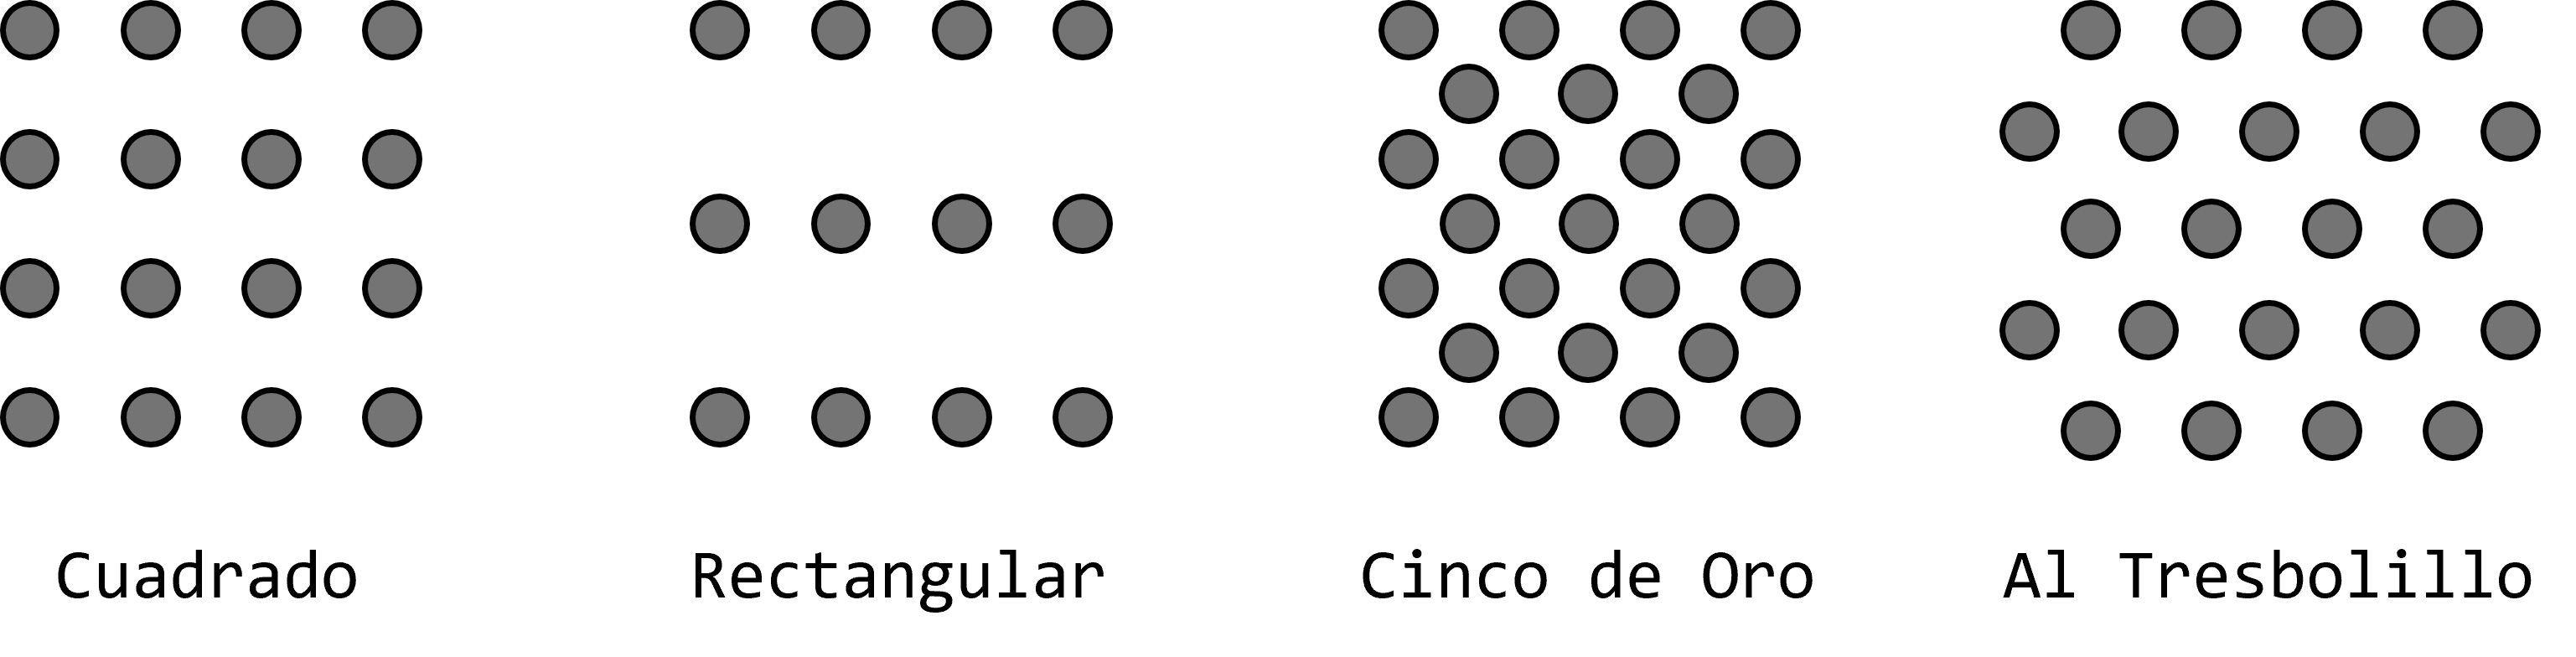
\includegraphics[width=0.8\linewidth]{Sources/figura1.png}
                \caption{Main plantation frames.}\label{fig:MarcosDePlantación}
            \end{figure}
            
            Tres bolillos or trebolillo is one of the most used planting systems today. This is based on planting in the shape of equilateral triangles, where each vertex represents the place where a plant will be planted, this way we ensure that each plant has the same separation with all its neighbors. The reason why this system is so widely used is because it allows better use of the planting space, allowing 17\% (\cite{Anonimo1}) more plants to be planted compared to the rectangular planting method; it also allows better control of erosion and light collection, since the shadow of one tree is not projected directly on others (\cite{Iglesias}).
            To use this system, it is necessary to first decide how much distance there will be between each plant, which depends on its characteristics and the environment. Subsequently, the distance between each groove (rows) is calculated, which is equal to the height of the equilateral triangle (\cite{Guerrero2018}).

            \begin{equation}
                h = d\cos{30}
            \end{equation}
            \\
            where h is the distance between rows and d the distance between each tree. On the other hand, it is possible to know the number of plants that fit in a given space using trigonometry in the following way (\cite{Carbo}):

            \begin{equation}
                n = \frac{A}{d^2 \cos{30}}
            \end{equation}
            where n is the number of plants, A is the area of available land and d is the distance between each plant.


% --------------------------------- Problema de Ruteo de Vehículos ---------------------------------
            %\vspace{0.5cm}
            \subsubsection{Routing Vehicule Problem (RVP)}
            The Vehicle Routing problem is one of the most studied combinatorial optimization problems in recent decades, mainly due to its relevance for the industry. This consists of determining a set of routes for a fleet of vehicles that depart from one or more depots to satisfy the demand of geographically dispersed customers \parencite{Sarmiento2014}. Of course, there are a large number of constraints that can be considered in addition to meeting demand \parencite{Toth2002}:

            \begin{itemize}
                \item Each vehicle has a limited capacity (capacitated VRP).
                \item Each client must be visited in a certain time slot (VRP with time windows).
                \item Multiple supply points (multiple depots VRP).
                \item Customers can be served by multiple vehicles (VRP with split supply).
                \item Some variables in the problem are random (stochastic VRP).
                \item Deliveries must be made on certain days (periodic VRP).
            \end{itemize}

            Typically, this problem is addressed by focusing on a single objective, commonly minimizing the distance traveled or \textit{cost} of routes, minimizing the number of vehicles used to satisfy all customers, or minimizing the total transportation time \parencite{Toth2002, García2010}.

            \subsubsection*{Ideas for the Routing Vehicule Problem Formulation}
            The road network is generally described with a graph, the arcs represent sections or road sections and the vertices correspond to the clients. Each arc has an associated cost that represents the length, travel time, or some function of these \parencite{García2010}.

            To solve this problem exactly, there are generally three approaches:
            \begin{itemize}
                \item \textit{Formulation with vehicle flow}: Uses integer variables associated with each arc that count the number of times a vehicle crosses it. Generally used for basic VRP.\@ This is very functional for cases where the cost of the solution can be expressed as the sum of the costs associated with the arcs \parencite{Toth2002}.
                \item \textit{Formulation with goods flow}: Uses additional integer variables associated with the arcs or edges that represent the flow of goods along the paths traveled by the vehicles \parencite{Toth2002}.
                \item \textit{Formulation as a partition problem}: These have an exponential number of binary variables, each of which is associated with the use (or non-use) of a different feasible path. Thus, the VRP is formulated as a set partition problem that searches for the set of routes with minimum cost that satisfy the constraints of the VRP \parencite{Toth2002}.
            \end{itemize}

            \subsubsection{Models to Solve the Vehicle Routing Problem (RVP)}
             Below are the formulations of some models used to study this type of problems.

            \subsubsection*{Model with Lower Limit of Vehicles \parencite{Larraín2021, Toth2002}}
             Based on the formulation of the Traveling Agent Problem by Dantzig, Fulkerson and Johnson. Let $G=(V, A)$ be a complete directed graph, with costs $c_a$. The set $N={1, 2, \ldots , n}$ represents the clients, with demand $q_i$. Node zero (not included in $N$), represents the warehouse, where there are $K$ vehicles of capacity $Q$ to visit customers in $N$. We define $V:=N \cup \{0\}$ and $A$ the set of arcs that join the elements in $V$. Finally, the binary variables $x_a$ indicate whether the arc $a$ is used in the solution. The objective function to minimize would be the sum of the products of the cost of the arcs and the binary that determines whether they are used or not. Posed as an integer programming problem:
            
            \begin{equation}
                Minimize \sum_{(i, j) \in A} c_{ij} x_{ij}
            \end{equation}

            \[s.a. \sum_{j \in \delta^+ (i)} x_{ij} = 1, \hspace{0.5cm} \forall i \in N\]
            \[\sum_{i \in \delta^- (j)} x_{ij} = 1, \hspace{0.5cm} \forall j \in N\]
            \[\sum_{j \in \delta^+ (0)} x_{0j} = K\]
            \[\sum_{(i,j) \in \delta^+ (S)} x_{ij} \geq r(S),  \hspace{0.5cm} \forall S \subseteq N, S \neq \emptyset\]
            \[x_{ij} \in {0, 1}, \hspace{0.5cm} \forall (i, j) \in A\]

            Where $\delta^+ (i)$ represents the arcs leaving node $i$ in $G$; and similarly $\delta^- (i)$ represents the arcs going towards the node $i$. $r(S)$ is a function that returns a lower bound corresponding to the minimum number of vehicles needed to satisfy the demand of the nodes in the subset $S$. For example, an acceptable limit would be:
            
            \[r(S) = \frac{\lceil \sum_{i\in S} q_i \rceil}{Q}\]
            
            This limit is quite intuitive: ceiling of the quotient between the sum of the demand in a subset of nodes $S$ and the capacity of the vehicles, this gives us a minimum (although surely not viable) for the number of vehicles necessary to satisfy the demand of subset $S$.

            The first two constraints specify that for each node (excluding the repository) there must be exactly one input arc and one output arc. It is important to note that these restrictions imply that the demand of a node cannot be shared by more than two vehicles.
            
            The third constraint specifies that exactly $K$ arcs must emerge from node zero (the depot), one for each vehicle. The fourth constraint requires that the arcs departing (directed toward an external node) from any subset of nodes $S \subseteq N$, which is equivalent to the number of vehicles proposed to be used to satisfy the demand of the nodes in $ S$, is greater than or equal to a lower bound $r(S)$. This restriction is responsible for avoiding \textit{sub-tours} (tours that do not include the deposit, therefore, are invalid). And finally, the fifth constraint defines the binary nature of $x_{ij}$.

            \subsubsection*{Model with MTZ Constraints \parencite{Larraín2021, florez2017}}
            This formulation bases its restrictions on the work of Christofides, Mingozzi and Toth. The approach is almost identical to the previous model, but the logic changes to avoid \textit{sub-tours}. Let $G=(V, A)$ be a complete directed graph, with costs $c_a$. The set $N={1, 2, \ldots , n}$ represents the customers, with demand $q_i$. Node zero (not included in $N$), represents the warehouse, where there are $K$ vehicles of capacity $Q$ to visit customers in $N$. We define $V:=N \cup \{0\}$ and $A$ the set of arcs that join the elements in $V$. The variables $q_i$ are added, which represent the total load that the delivery vehicle has distributed until the moment it leaves the node $i$. Finally, the binary variables $x_a$ are defined, indicating whether the arc $a$ is used in the solution. Posed as an integer programming problem:

            \begin{equation}
                Minimize \sum_{(i, j) \in A} c_{ij} x_{ij}
            \end{equation}

            \[s.a. \sum_{j \in \delta^+ (i)} x_{ij} = 1, \hspace{0.5cm} \forall i \in N\]
            \[\sum_{i \in \delta^- (j)} x_{ij} = 1, \hspace{0.5cm} \forall j \in N\]
            \[\sum_{j \in \delta^+ (0)} x_{0j} = K\]
            \[u_i - u_j + Qx_{ij} \leq Q - q_j, \hspace{0.5cm} \forall (i, j) \in A(N)\]
            \[q_i \leq u_i \leq Q, \hspace{0.5cm} \forall i \in N\]
            \[x_{ij} \in {0, 1}, \hspace{0.5cm} \forall (i, j) \in A\]

            Where $\delta^+ (i)$ represents the arcs leaving node $i$ in $G$; and similarly $\delta^- (i)$ represents the arcs going towards the node $i$. $A(N)$ represents the set of arcs that join the nodes in $N$.

            Almost all constraints are shared with the previous model, except the fourth and fifth, which are responsible for avoiding \textit{sub-tours}, and it is worth explaining the logic behind it. Note that the fourth constraint can be subdivided into two cases depending on whether $x_{ij}$ is $0$ or $1$. These are:

            \[x_{ij} = 1 \hspace{0.5cm} \implies \hspace{0.5 cm} u_j \geq u_i + q_j\]
            \[x_{ij} = 0 \hspace{0.5cm} \implies \hspace{0.5 cm} u_i - u_j \leq Q - q_j\]

            In the first case, the constraint requires that, for an arc $(i, j)$, the shared load accumulated up to the node $j$ is greater than or equal to the shared load accumulated up to the node $i$ visited just before plus the demand of node $j$. In the opposite case, the restriction is always satisfied, becoming redundant (on purpose), since $u_i - u_j \leq 0$ and $Q - q_j \geq 0$ (remember that in this model the vehicles do not share nodes).

            The advantage of using this model compared to the lower bound model is that the \textit{sub-tours} restriction of the latter has exponential cardinality with respect to the number of nodes; while with the MTZ model the cardinality is polynomial, saving computing time \parencite{García2010}.

            \subsubsection*{Sets Partition Model \parencite{García2010, Toth2002}}
            This model was originally proposed by Balinski and Quandt \parencite{Balinski1964}. Returning to part of the previous approaches, let $\mathcal{R} = \{R_1, R_2, R_3 \ldots , R_s\}$ be the set of all feasible routes or circuits in $G$, each route is assigned a cost $\gamma_j$. Binary variables $a_{ij}$ are defined, which is worth $1$ only if node $i$ is visited (or covered) by route $R_j$. Binary variables $x_j$ are also defined, which are worth $1$ only if path $R_j$ is used in the optimal solution. It is posed as an integer programming problem in the following way:

            \begin{equation}
                Minimize \sum_{j=1}^s \gamma_j x_j
            \end{equation}

            \[s.a. \sum_{j=1}^s a_{ij} x_j = 1, \hspace{0.5cm} \forall i \in N\]
            \[\sum_{j=1}^s x_j = k \]
            \[x_j \in \{0, 1\}, \hspace{0.5cm} \forall j \in \{1, 2, \ldots , s\} \]
            \[a_{ij} \in \{0, 1\}, \hspace{0.5cm} \forall i \in V, \hspace{0.25cm} j \in \{1, 2, \ldots , s\} \]

            The first constraint requires that each client is visited by exactly one of the circuits of $\mathcal{R}$. The second constraint requires that exactly k circuits of $\mathcal{R}$ are chosen. This formulation is very general, but easily moldable, although it has the disadvantage that it requires providing the exponential growth set $\mathcal{R}$ in advance.






    % ---------------------------------- DEFINICIÓN DEL PROBLEMA ----------------------------------
    \section{Problem Definition}
    It seeks, through a mathematical model and/or a heuristic algorithm, to provide the staff of Comisión Nacional Forestar (CONAFOR) with a method to optimally plan the routes necessary to comply the number of individuals that will be necessary for each section of the hectares (Figure~\ref{fig:tablaDePlantas}). Given the type of problem, it is possible to create this plan through linear programming, posing it as a \textit{vehicule routing problem}, representing the polygons and the base of operations as nodes joined by arcs with a determined cost.

        \subsection{Sets}
        \begin{itemize}
            \item $N$ is the set that represents the polygons (demanding nodes).
            \item $V$ is the set $N\cup {0}$ where the element $0$ represents the deposit or base.
            \item $A$ is the set of arcs that join the elements in $V$.
            \item $K$ is the set of vehicles (or trips that can be made).
        \end{itemize}
        
        \subsection{Parameters}        
        \begin{itemize}
            \item There is a work schedule of 8 hours per day.
            \item The truck has capacity for 524 plants, divided into certain proportions (see Figure~\ref{fig:tablaDePlantas}). This measurement is equivalent to 1 \textit{hectare of plants}.
            \item The time it takes to fully load and unload a van is 30 minutes.
            \item There are 30 claimant polygons with an area of 182.99 hectares in total.
            \item A speed of 20 kilometers per hour is considered for trucks.
            \item The cost per kilometer of gasoline is 0.1 liters of gasoline.
            \item \(c_{ij}\) is the distance in km between node $i$ and node $j$.
            \item \(Q\) the capacity of the truck.
            \item \(d_{ij}\) the distance between polygon $i$ and $j$.
        \end{itemize}
        
        \subsection{Variables}
        \begin{itemize}
            \item Let $x_{ijk}$ be a binary that only takes the value 1 if vehicle $k$ travels through the arc $(i,j)$.
            \item Let $w_{ijk}$ be the amount of resource transported by vehicle $k$ through the arc $(i,j)$.
            \item Let $u_{ik}$ be an ordinal number corresponding to the chronological position taken by the node $i$ in the route of the vehicle $k$, taking the value 0 if said node is not used.
        \end{itemize}

        \begin{figure}[ht]
            \centering
            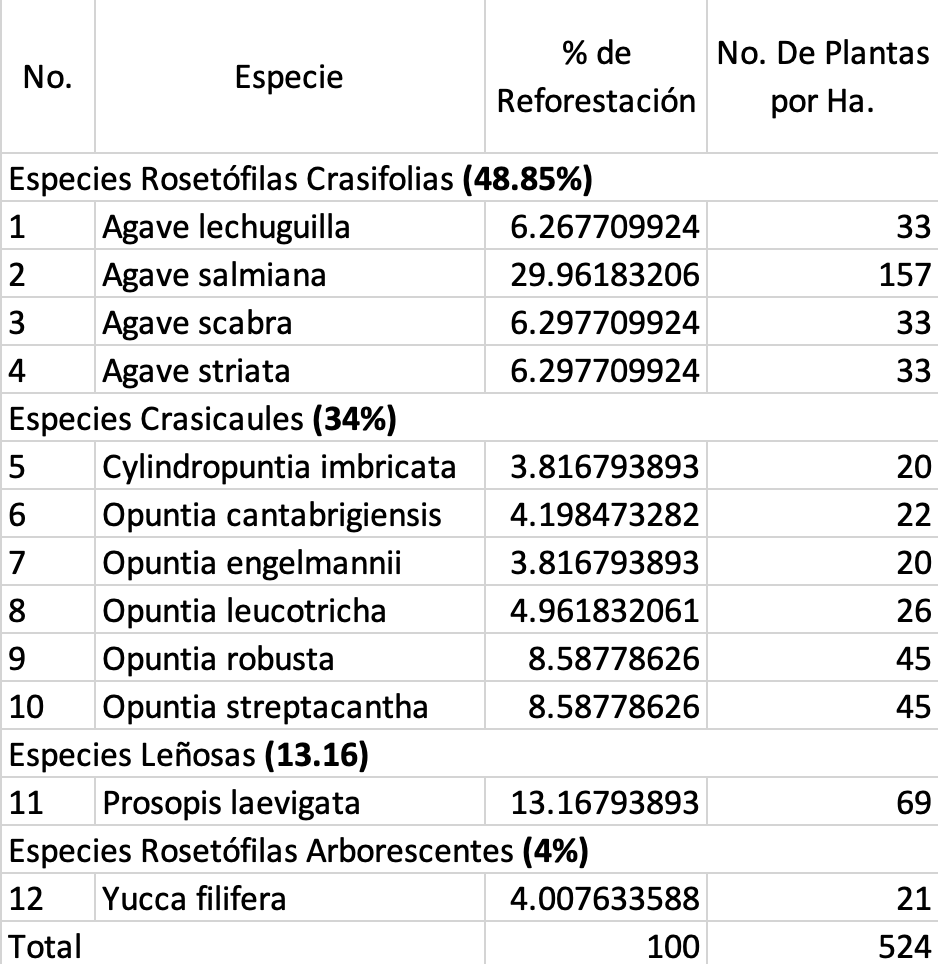
\includegraphics[width=0.35\linewidth]{Sources/TablaDePlantas.png}
            \caption{Tabla de Plantas requeridas por hectárea.}\label{fig:tablaDePlantas}
        \end{figure}
        
        
        

    % -------------------------------------- ENTREGA 2 --------------------------------------
    \section{Methodology}
        It is possible to model the reforestation process by implementing a directed graph $G=(V,A)$ made up of vertices and edges, the vertices representing the discharge points and the edges representing the distance between each of them.

        After a brief analysis, it can be observed that the project has many similarities with VRP (Vehicule Routing Problem) models, specifically VRP with split deliveries. These problems are characterized by having a source node, which supplies resources to all other nodes, which can be satisfied in several deliveries. From the source node, k vehicles depart, which can have identical or different load capacities \parencite{Dror}.

        For this model, given the limited information on the paths available, it was decided to implement the Euclidean distance as the cost of taking each edge. These costs are represented by the parameter \textit{c (i,j)}. On the other hand, since the number of vehicles available is not known, it was decided to set the number of vehicles as the minimum number of cycles needed to meet all the demands, defining a cycle as one that starts leaving the origin node and ends arriving at the same node. 

        To obtain the distances between the nodes, we used the image with the geographic location of the polygons provided by CONAFOR, the scale in meters presented in said image was used and a Python code was implemented that allowed us to obtain the distance between each node by simply entering the approximate coordinate of the center of each one.
        
        During the modeling process, we realized that, if we assume that all vehicles used have the same capacity, many of the nodes need one or more fully loaded trucks to be satisfied, that is, it is necessary to make multiple routes where the vehicles leaves the origin node, arrives at the node to be supplied, unloads all the cargo it carries and returns to the origin node. After this, we realized that most of the delivery cycles can be easily determined just by rounding the demand to the nearest lowest integer. For example, if a node has a demand of 6.28 and the vehicles capacity is 1, the model will always carry 6 fully loaded trucks, leaving the node with only the decimal part to supply. The order in which these routes are made does not change the cost and calculating the latter does not require great computational capacity.

        It can then be seen that the problem is reduced to determining the routes to follow to supply the decimal parts of the demands, thus reducing the complexity of the problem. For this simplified model it can be observed that the number of nodes is reduced to 26, since there are 5 that have integer demands.

        Since the aim is to optimise the time it takes for the vehicles to supply the requested demands, it is necessary to consider the speed at which these vehicles move. Being heavy-duty trucks, these tend to have low acceleration and speed, mainly when dealing with unpaved roads, as in this case study. We consider an average speed of 20 km/h, since there are no established roads on most of the routes and the reforestation area has a uniform altitude.

        To obtain an optimal solution, a mixed linear programming mathematical model is first proposed (See Section~\ref{ModeloMatematico}). This model was executed in the GAMS modeling software and in Python with the help of the PuLP library. However, the proposed model is too complex for the license we have in GAMS, while in Python, the model exceeds the time limit.

        Because of this, a heuristic solution is proposed (See Section~\ref{MetodoHeuristico}), which, through Python code, allows obtaining a solution very close to the optimal one, using much less memory and execution time.

    \section{Mathematical Model}\label{ModeloMatematico}

        \subsection{Definitions}
        \subsubsection{Sets}
        Set $N=\{1, 2, \ldots , n\}$ represents the clients. It is defined $V=N \cup \{0\}$, where $0$ represents the depot. $A$ is the set of arches that join the elements in $V$. $A'$ is the set of arches that join the elements of $N$. With the above, $G=(V, A)$ is a directed and complete graph of nodes $V$ and edges $A$. It's defined $K = \{1, 2, \ldots, m\}$, representing the vehicles (or the different routes that must be taken).

        \subsubsection{Parameters}
        Let $n \in \mathbb{N}_0$ the number of customers, each with a demand of $q_i : i \in N$. Let $m \in \mathbb{N}$ the maximum number of vehicles (or independent routes) available, all of them with capacity $L \in \mathbb{R}^+$. Note that a lower bound can be placed for $m \geq (\sum q_i) \div Q$. The graph $G$ has costs per unit $c_{a} : a \in A$. Let $\mathcal{M}$ a constant large enough to relate continuous and binary variables in constraints that is at least equal to the maximum demand. Let $v$ a constant corresponding to the average speed of vehicles in meters/hour, and $t$ a constant corresponding to the charging or discharging time measured in hours.

        \subsubsection{Variables}
        Let $x_{ijk}$ a binary variable that takes value $1$ if vehicle $k$ uses the edge $(i, j)$ on his route, or take value $0$ if it's not used. Similarly, $w_{ijk} \geq 0$ represents the amount of material transported by the vehicle $k$, leaving node $i$ and to deliver to the node $j$. Finally $u_{ik} \in \mathbb{Z}^+$ takes a value corresponding to the order in which the node $i$ is visited by the vehicle $k$.

        \subsection{Definition as a Linear Programming Problem}
        Posed as a linear programming problem, it can be written as follows:
            
            \begin{equation}
                Minimizar \hspace{0.5cm} v^{-1} \sum_{i \in V} \sum_{j \in V} \sum_{k \in K} c_{ij} x_{ijk} + 2t \sum_{i \in V} \sum_{j \in V} \sum_{k \in K} w_{ijk} \hspace{0.5cm} : i \neq j
            \end{equation}

        \[Sujeto\hspace{0.2cm} a \hspace{0.5cm} \sum_{j \in V} x_{ijk} - \sum_{j \in V} x_{jik} = 0 \hspace{0.5cm} : i \neq j \hspace{0.5cm} \forall i \in V, \hspace{0.5cm} k \in K\]

        \[\sum_{j \in N} x_{0jk} = 1 \hspace{0.5cm} \forall k \in K\]

        \[\sum_{i \in V} \sum_{j \in V} w_{ijk} \leq L \hspace{0.5cm} : i \neq j \hspace{0.5cm} \forall k \in K\]

        \[\sum_{i \in V} \sum_{k \in K} w_{ijk} \geq q_j \hspace{0.5cm} : i \neq j \hspace{0.5cm} \forall j \in N\]

        \[u_{ik} - u_{jk} + n x_{ijk} \leq n - 1 \hspace{0.5cm} : i \neq j \hspace{0.5cm} \forall i,j \in N, \hspace{0.2cm} k \in K\]

        \[w_{ijk} \leq \mathcal{M} x_{ijk} \hspace{0.5cm} \forall i,j \in V, \hspace{0.2cm} k \in K\]

        \[x_{ijk} \in {1, 2} \hspace{0.5cm} \forall i,j \in V, \hspace{0.2cm} k \in K\]
        
        \[w_{ijk} \geq 0 \hspace{0.5cm} \forall i,j \in V, \hspace{0.2cm} k \in K\]

        The objective function to be minimized is the sum of the product of the costs per arc and the binary that indicates whether it was used or not, multiplied by the reciprocal of the speed, all of this representing the time invested in traveling distances; plus the sum of all the loads delivered multiplied by $2t$, which is the loading/unloading time, which is assumed to vary linearly depending on the number of plants to be unloaded. The first constraint is to conserve the flow of vehicles. The second constraint ensures that all cars pass through node zero (depot). The third constraint corresponds to the maximum load of each vehicle. The fourth constraint is to satisfy the demands of each customer. The next constraint is used to avoid subtours, by assigning each node a positive integer corresponding to the order in which they are visited by each vehicle. The last three constraints are about the nature of the variables: $x_{ijk}$ must equal zero only if $w_{ijk}$ is equal to $0$, and must be equal to $1$ otherwise. $x_{ijk}$ is a binary variable. $w_{ijk}$ must be greater than or equal to zero to avoid transporting a negative amount of material (plants).

        \section{Heuristic Method}\label{MetodoHeuristico}
        For the heuristic method, we chose to use a greedy heuristic algorithm, which starts by completely supplying the demand of the node furthest from the depot, and then unloads the remaining resource at the node closest to the one previously visited. This makes deliveries more efficient, because having visited and completely supplied the furthest node, no matter where you move, you always get closer to the base. Because the furthest customers are the ones that generate the most costs, this algorithm allows us to reduce the number of times it is necessary to travel to a distant node.
        
        \subsection{Preliminary Results}
        As explained above, the reduced problem consists of satisfying those polygons where the demand is non-integer, so the solution implemented with the heuristic method focused only on these nodes, 26 in total, counting the node that represents the base (demand 0).

        In total, we obtained 15 different routes needed to satisfy the demand of the decimal part of the nodes, shown in Table~\ref{ParteDecimal}. Likewise, two of the routes of the proposed model are shown graphically (see Figure~\ref{fig:RutasDeEjemplo}). The rest of the routes can be seen in the appendices.

        \begin{figure}[ht]
            \begin{center}
                \subfloat[Route 1.]{
                    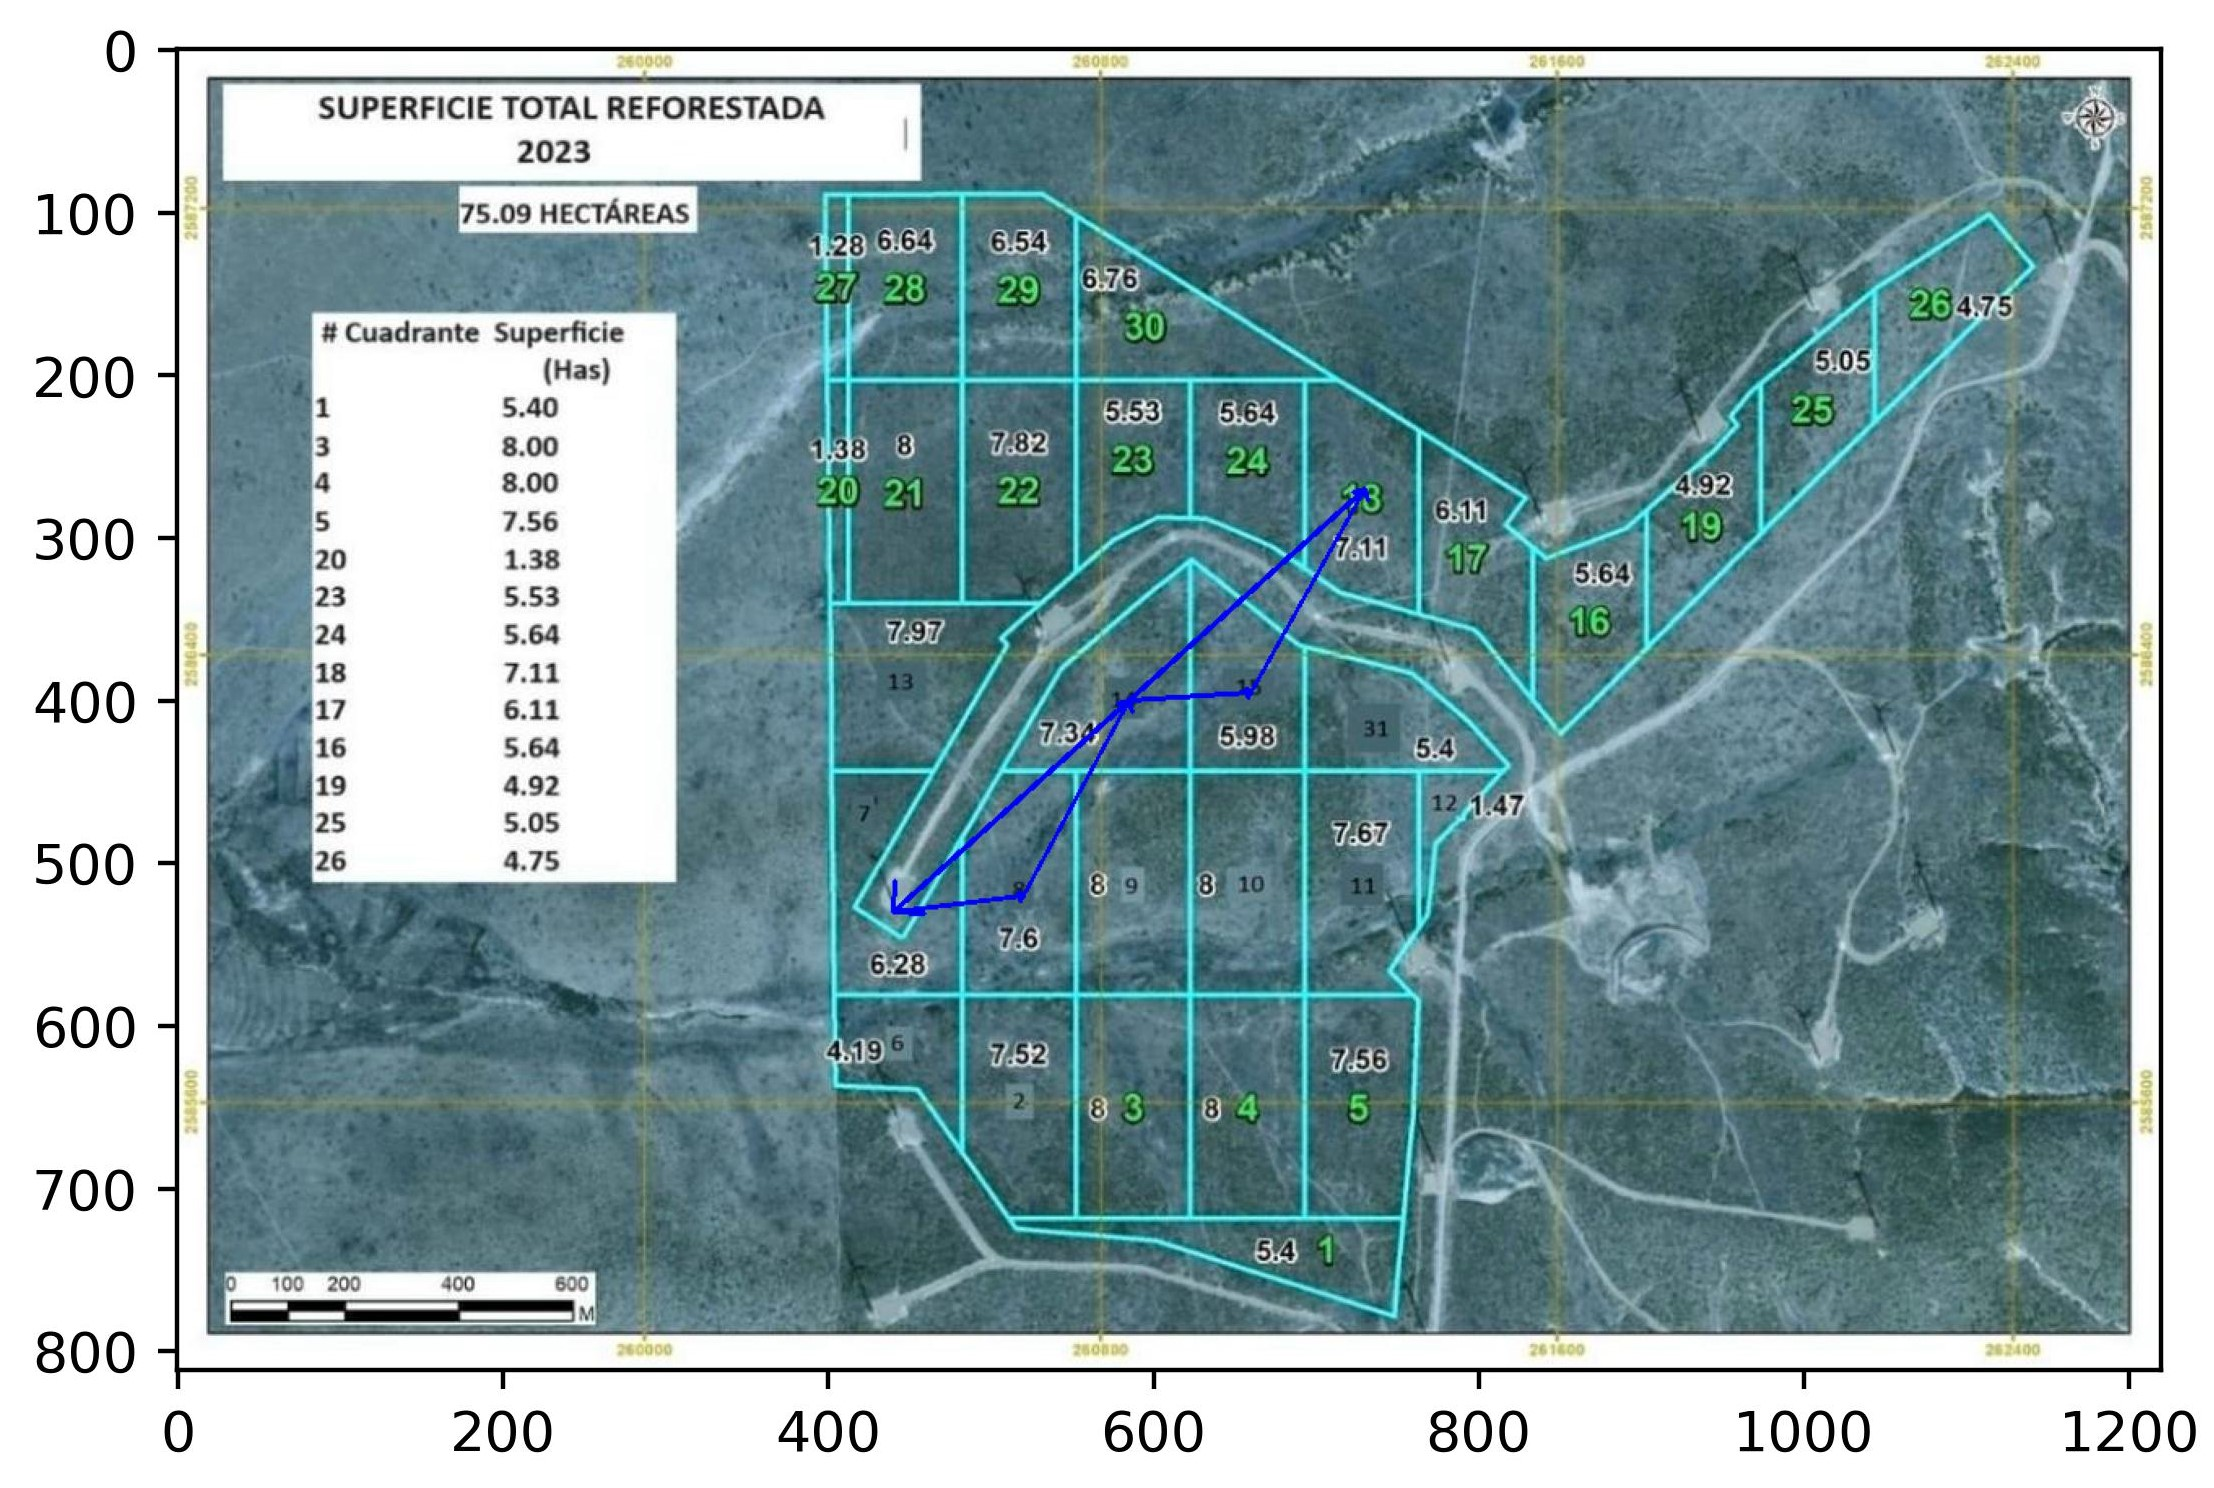
\includegraphics[width=0.48\linewidth]{Sources/Ruta_3.jpg}
                }
                \subfloat[Route 13.]{
                    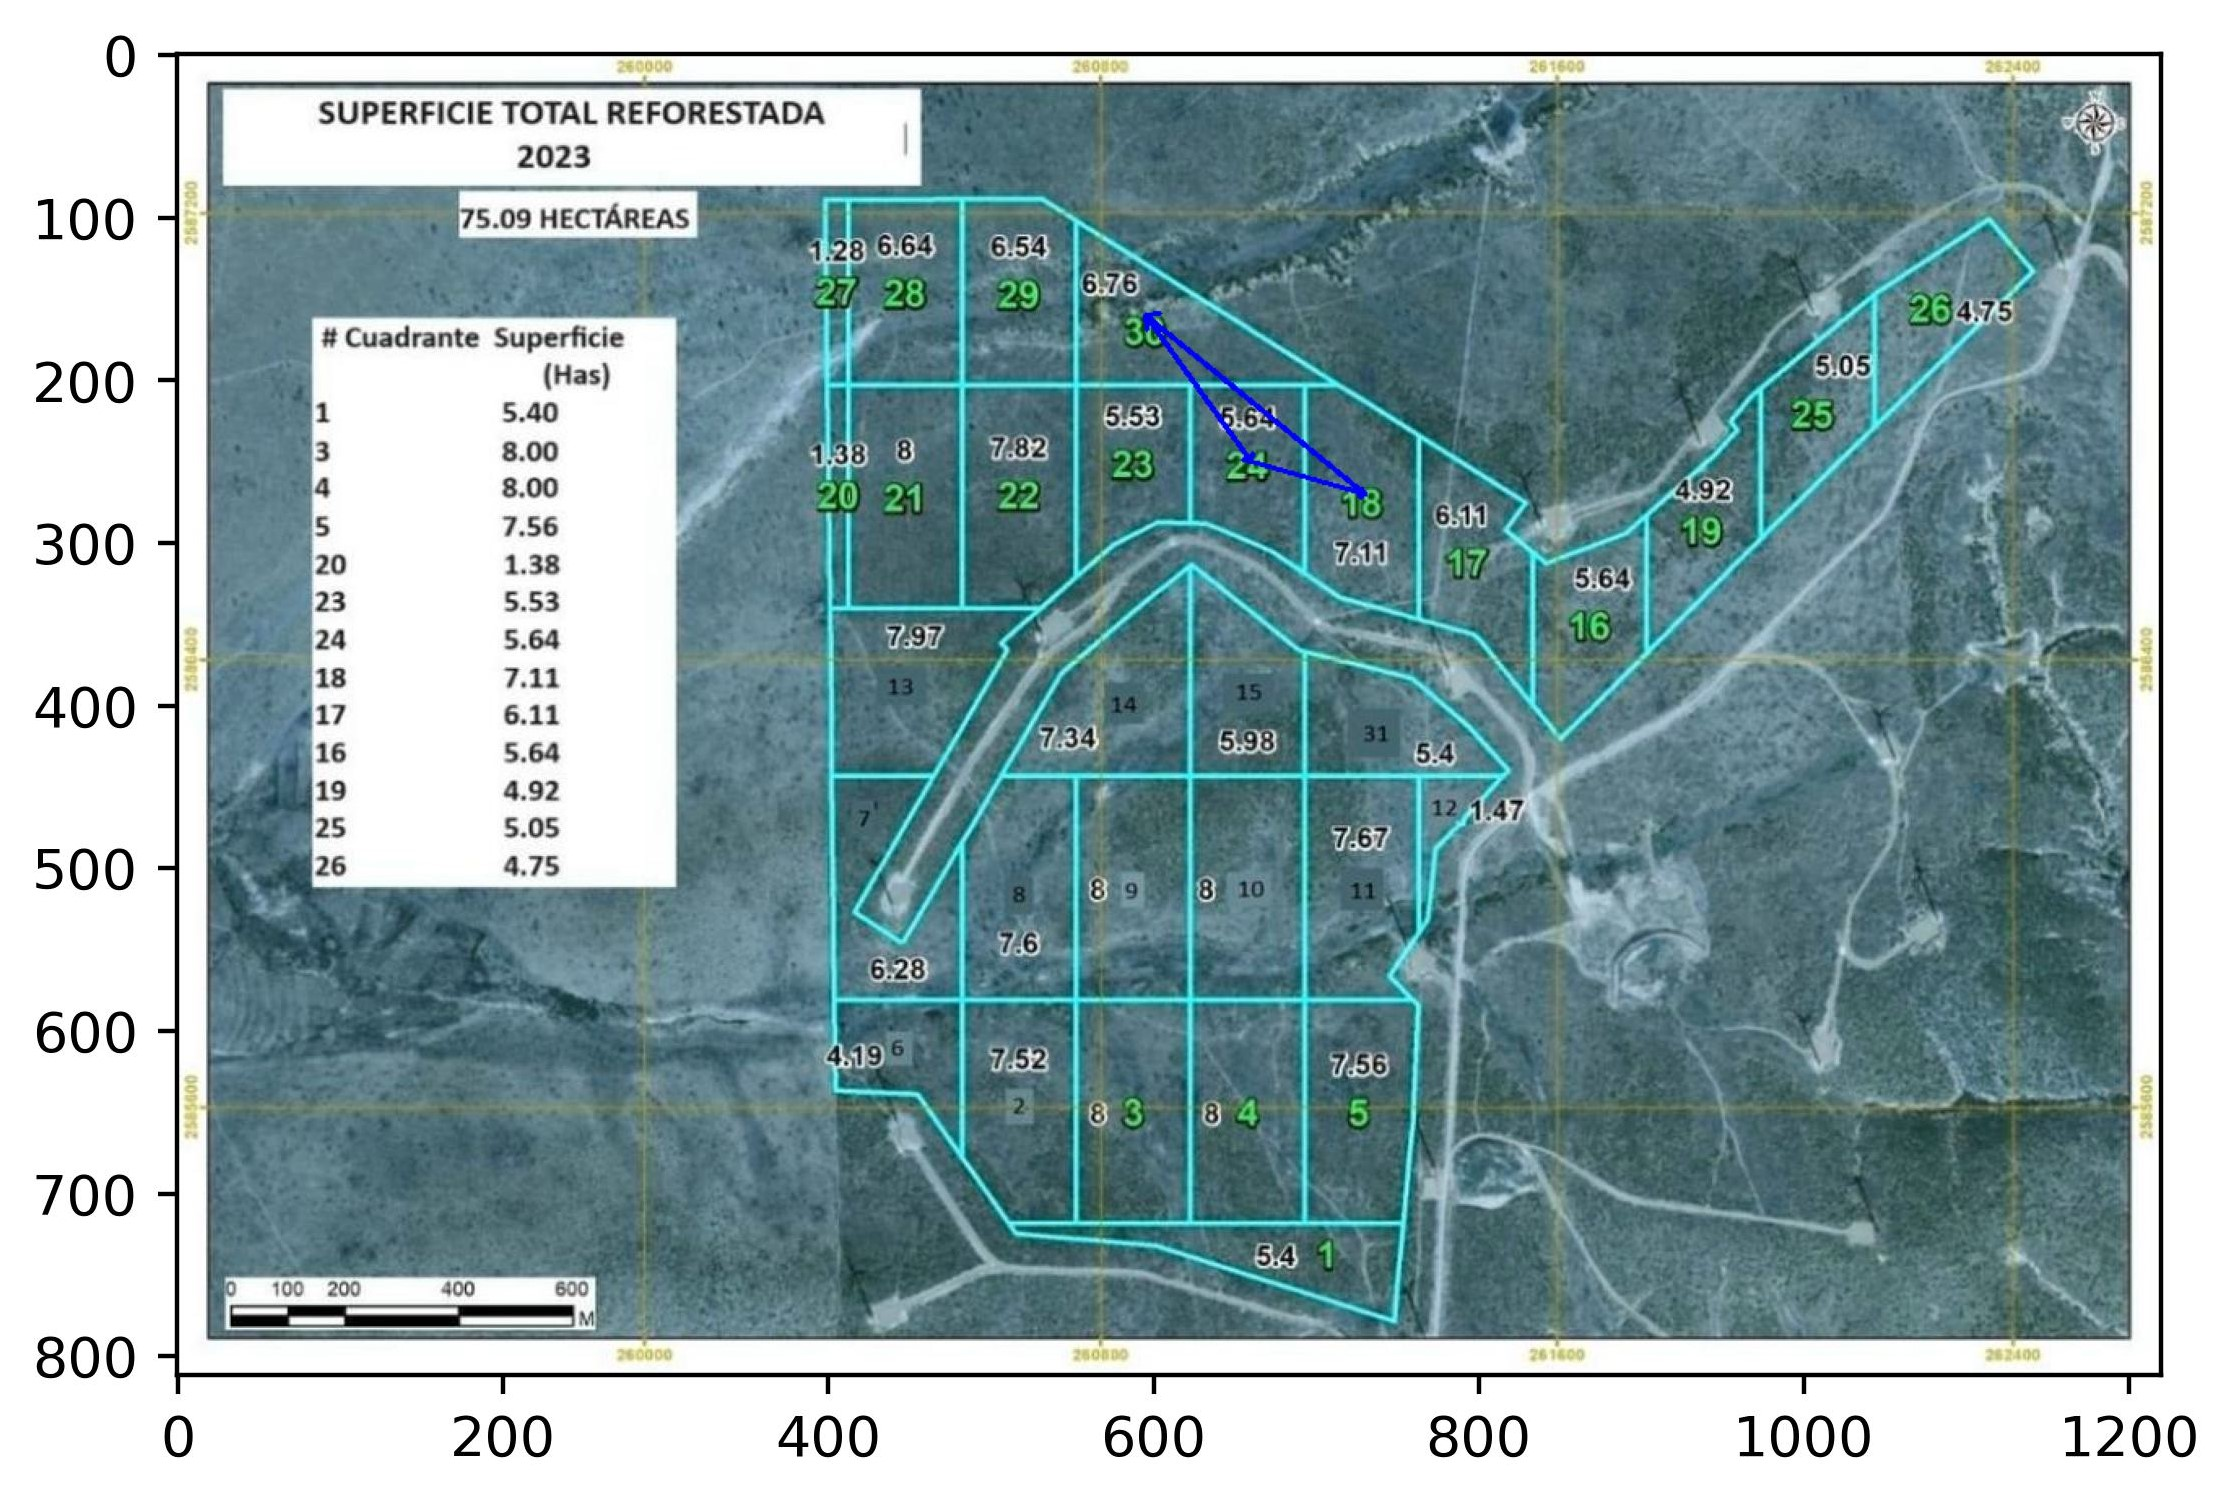
\includegraphics[width=0.48\linewidth]{Sources/Ruta_13.jpg}
                }
                \caption{Some routes that are part of the heuristic solution.}\label{fig:RutasDeEjemplo}
            \end{center}
        \end{figure}
        

        The total cost of the decimal part of the routes is 15.001 hours, while the total cost in hours of the integer part of the routes is 182 hours. This adds up to a total of 197 hours, or 24.7 working days.
        
    From the routes in Table 1, a route distribution was made, which considers that once a node has been visited, it has to fill its entire part as soon as possible, and nodes that have been fully filled should not be passed over. These routes were planned with an 8-hour work day, as well as the use of only one van. Once ordered, the algorithm took 26 work days (Table~\ref{DistribucionViajes}).




    % -------------------------------------- ENTREGA 3 --------------------------------------
    \section{Experimentación y Resultados}
    La experimentación tanto para el modelo matemático como para el metodo heuristico se llevó a cabo en un computadora con las siguientes caracteristicas:
    \begin{itemize}
        \item \textbf{Modelo de la PC:} Dell G15 5520
        \item \textbf{Sistema operativo:} Windows 11.
        \item \textbf{Capacidad de disco duro:} 512GB
        \item \textbf{Memoria Ram:} 16GB\@.
        \item \textbf{Tipo de procesador:} 12th Gen Intel (R) Core (TM)
        \item \textbf{Numero de nucleos:} 7
        \item \textbf{Software utilizado y versión:} Para el modelo matemático se usó la librería PuLP 2.8.0 de Python en combinación con la licencia de CPLEX IBM.\@Para el metodo heuristico se hizo uso de Pandas 2.2 en Python.
    \end{itemize}

        \subsection{Tamaño del problema}
            \subsubsection{Nodos y Arcos}
            El problema original, en su parte decimal, cuenta con 26 nodos (excluyendo 5 nodos cuya parte decimal es cero), obteniendo a su vez 676 arcos.
            \subsubsection{Variables}
            El modelo suma un total de 20670 variables de decisión, tomando en cuenta tres grupos de variables: 
            \begin{itemize}
                \item $x_{ijk}$ una variable binaria que toma el valor de 1 si el vehículo $k$ utiliza el arco $(i,j)$ en su ruta y 0 si no lo utiliza. Ya que se consideran variables distintas para cada uno de los 15 vehículos a utilizar, existen 10140 variables de este tipo.
                \item $w_{ijk}$ representa la cantidad de material que transporta el vehículo $k$ para el arco $(i,j)$. Ya que se consideran variables distintas para cada uno de los 15 vehículos a utilizar, existen 10140 variables de este tipo.
                \item $u_{ik} \in Z^+$ toma un valor correspondiente al orden en el que el nodo $i$ es visitado por el vehículo $k$. Ya que existen 26 nodos y 15 vehículos a utilizar, existen 390 variables de este tipo.
            \end{itemize}
            

            \subsubsection{Parámetros}
            El modelo cuenta con un total de 707 parámetros, que son parte de la siguiente lista:
            \begin{itemize}
                \item $c_{ij}$ siendo el costo de viajar del nodo $i$ al nodo $j$, resulta en 676 parámetros, uno por arco.
                \item $q_i$ como la demanda del nodo $i$, resulta en 26 parámetros.
                \item $m$ como la mínima cantidad de rutas requeridas.
                \item $L$ siendo la capacidad de los vehículos.
                \item $t$ el tiempo que toma cargar o descargar.
                \item $M$ una constante de gran tamaño.
                \item $V$ la velocidad promedio de los vehículos.
            \end{itemize}

        \subsection{Resultados}
            \subsubsection{Problemas Reducidos}
            Para comparar los resultados entre el modelo matemático y el método heurístico con el fin de determinar si la cercanía de la solución heurística a la solución óptima es aceptable (menor al 1\%), se usaron tres tamaños de problema que el modelo matemático es capaz de resolver en tiempos razonables, probando en grupos de cinco muestras tomadas aleatoriamente: con 5 nodos (Tabla~\ref{5nodos}), otro con 10 nodos (Tabla~\ref{10nodos}), y un ultimo con 12 nodos (Tabla~\ref{12nodos}). Para garantizar la igualdad de condiciones entre las muestras, se asegura que no contienen otros nodos de demanda cero además de la base. Asimismo, se incluyen gráfica que permiten visualizar la diferencia de los tiempos de procesamiento de los 3 tamaños tanto para el modelo matemático como para el heurístico (Figura~\ref{GraficasTiemposProcesamiento}).

            \begin{table}[ht]
                \centering
                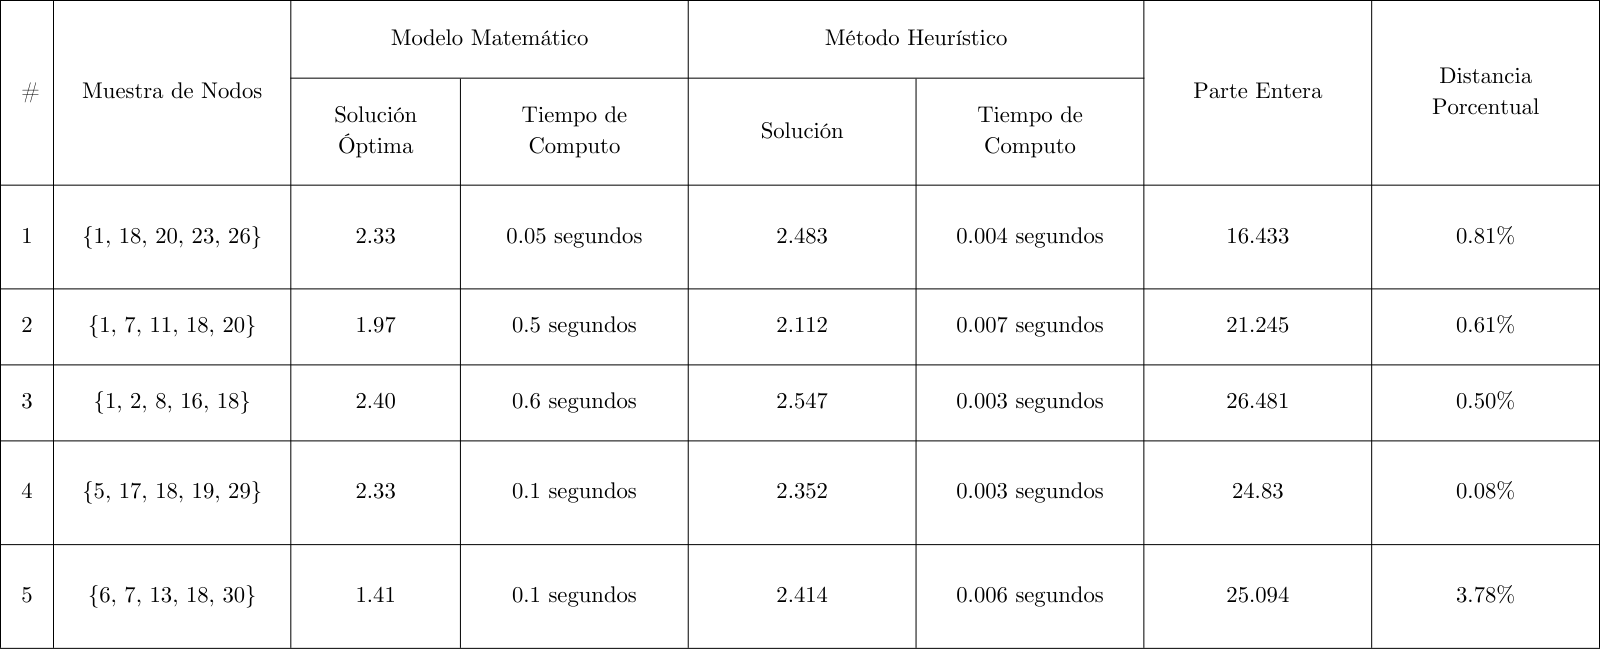
\includegraphics[width=1\linewidth]{Sources/Tabla1.png}
                \caption{Resultados para casos de prueba con cinco nodos.}\label{5nodos}
            \end{table}    

            \begin{table}[ht]
                \centering
                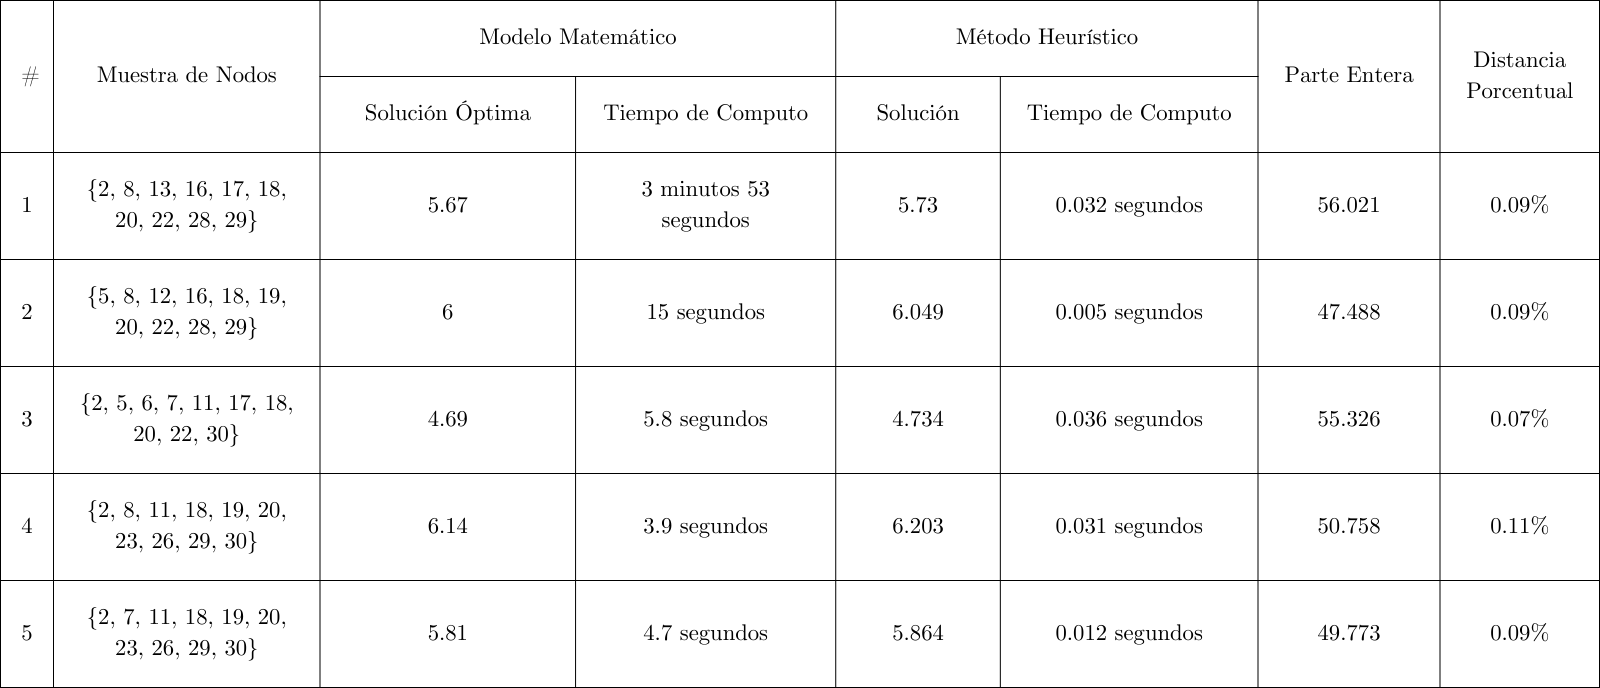
\includegraphics[width=1\linewidth]{Sources/Tabla2.png}
                \caption{Resultados para casos de prueba con diez nodos.}\label{10nodos}
            \end{table}
            
            \begin{table}[ht]
                \centering
                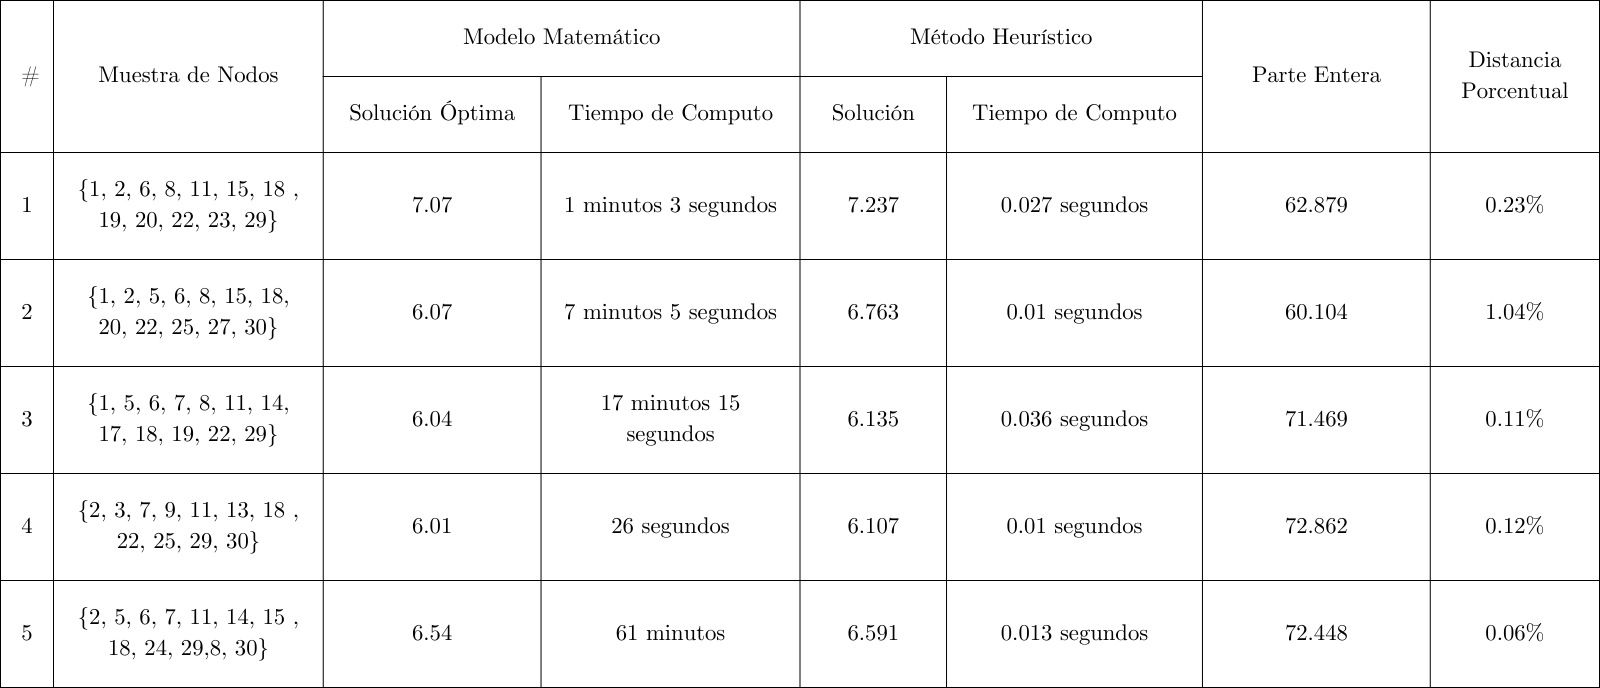
\includegraphics[width=1\linewidth]{Sources/Tabla3.png}
                \caption{Resultados para casos de prueba con doce nodos.}\label{12nodos}
            \end{table}

            \begin{figure}[ht]
                \begin{center}
                    \subfloat[Modelo matemático.]{
                        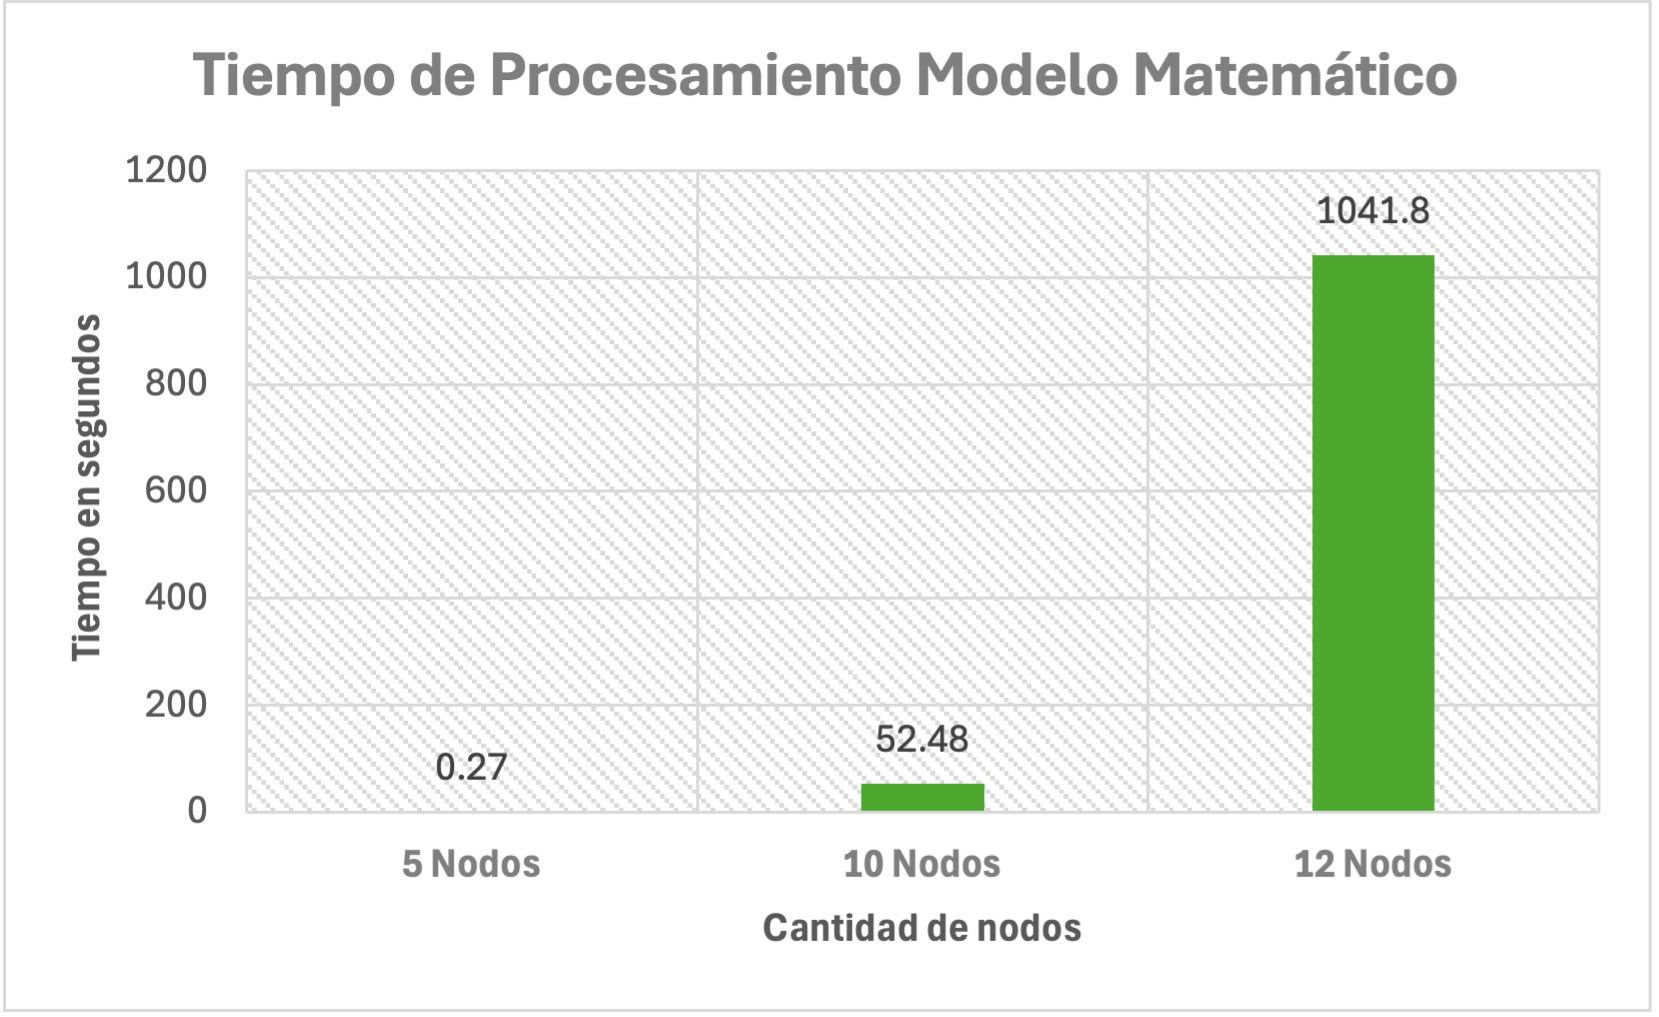
\includegraphics[width=0.48\linewidth]{Sources/graficaResultados1.png}
                    }
                    \subfloat[Metodo heurístico]{
                        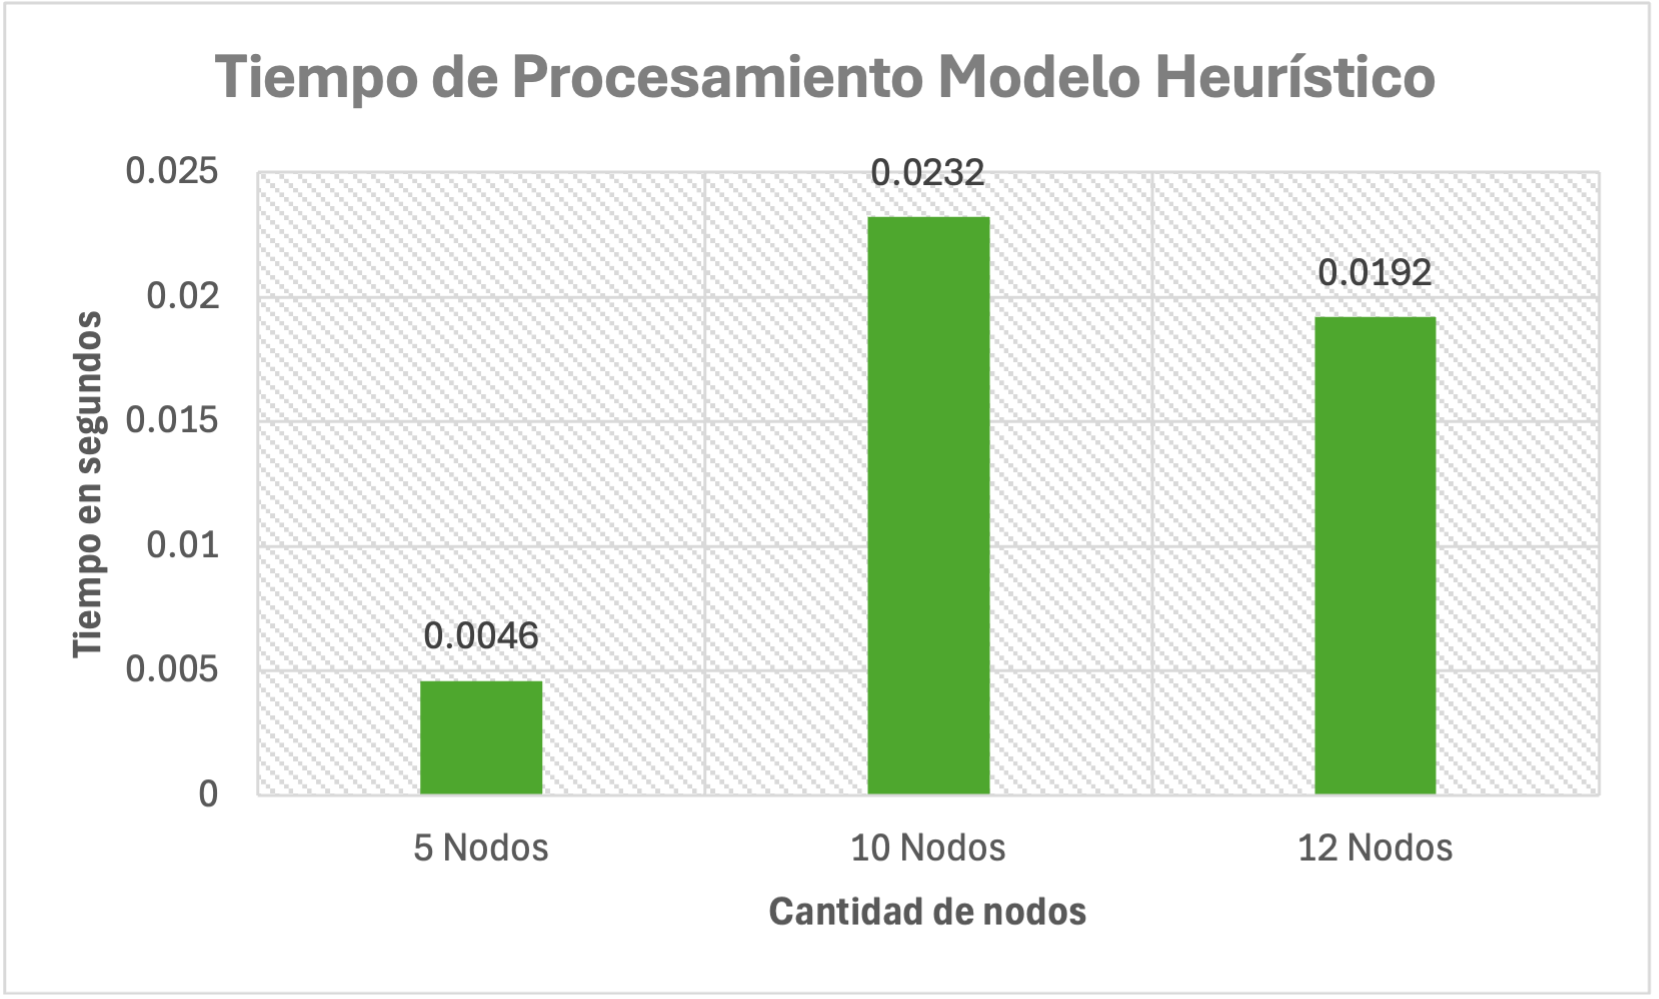
\includegraphics[width=0.48\linewidth]{Sources/graficaResultados2.png}
                    }
                    \caption{Tiempos de procesamiento para distintos tamaños de problema.}\label{GraficasTiemposProcesamiento}
                \end{center}
            \end{figure}

            \subsubsection{Problema Completo}
            Dado el tamaño de este problema, no fue posible resolverlo con el modelo matemático en un tiempo razonable (menor que 48 horas), por ello presentamos la solución obtenida mediante el método heurístico.
            Para la parte entera se tiene que serán necesarias 182.68 horas, mientras que para la parte decimal se requieren 15.18 horas. Por lo que el resultado de la función objetivo es:
            \[z^* = 197.86 \text{ horas}\]
            Equivalente a 25 jornadas laborales de 8 horas, si se considera un único vehículo, pero este tiempo puede reducirse si varios vehículos operan de forma paralela. Esta solución requiere 183 viajes, justamente los mínimos estimados a través de la cota inferior $\lceil \sum_{i} q_i \div L \rceil = 183$, prueba de que esta solución es factible.

    \section{Conclusiones}
    Dados estos resultados, se puede observar que el modelo matemático proporciona mejores resultados, pero el porcentaje de mejoría no es suficientemente alto como para asumir el costo computacional que requiere en problemas grandes. Es por esto que el resultado del problema completo solo se pudo llevar a cabo mediante el método heurístico. De igual manera, el bajo tiempo computacional que requiere este método, permite ajustes rápidamente en los parámetros y función objetivo, pudiendo obtener soluciones a instancias distintas del problema sin requerir un alto tiempo de espera para obtener una respuesta.
    

    \begin{table}[!htp]\centering
    \caption{Plan de Trabajo para la Parte Decimal de la Demanda}\label{ParteDecimal}
    %\scriptsize
    \begin{tabular}{lrrrrrr} \toprule
    \textbf{\#} & \textbf{Ruta} \\\midrule
    1 & base, 1, 5, 11, base \\
    2 & base, 6, 2, 8, base \\
    3 & base, 7, 8, 14, 15 base \\
    4 & base, 26, 25, 19, base \\
    5 & base, 27, 28, 29, base \\
    6 & base, 20, 22, base \\
    7 & base, 13, 22, base \\
    8 & base, 29, 30, base \\
    9 & base, 11, 12, base \\
    10 & base, 19, 16, base \\
    11 & base, 22, 23, 24, base \\
    12 & base, 12, 31, 15, base \\
    13 & base, 30, 24, base \\
    14 & base, 16, 17, base \\
    15 & base, 15, base \\
    \bottomrule
    \end{tabular}
    \end{table}

    El costo total de las rutas de la parte decimal es de 15.001 horas. Mientras que el costo total en horas de la parte entera de las rutas es de 182 horas. Sumando así un total de 197 horas, o 24.7 jornadas laborales.
            
    A partir de las rutas mostradas en la Tabla~\ref{ParteDecimal} se realizó una distribución de rutas, la cual considera que una vez visitado un nodo, este tiene que suplir su parte entera lo más pronto posible, así como no se debe pasar encima (atravesar geográficamente) de nodos que se hayan suplido totalmente, pues estos podrían estar ya plantados. Estas rutas fueron planeadas con una jornada laboral de 8 horas, así como el uso solamente de una camioneta. Una vez ordenadas, el algoritmo provee una solución que toma 26 jornadas laborales (Vea Anexos Tabla~\ref{DistribucionViajes}) para satisfacer a los 30 polígonos demandantes.




% -------------------------------------- Referencias --------------------------------------
\newpage
\printbibliography[title={References}]


% ----------------------------------------- ANEXOS ----------------------------------------
\newpage
\section{Anexos}

    \subsection{Plan de Trabajo Propuesto}
    Se incluyen detalles de cada viaje, así como el orden específico en el que debe realizarse para minimizar la cantidad de jornadas laborales requeridas y satisfacer exitosamente la demanda.
    
    \begin{table}[!htp]\centering
        \caption{Plan de Trabajo Completo para una Camioneta}\label{DistribucionViajes}
        \scriptsize
        \begin{tabular}{lrrrrrr}\toprule
        \textbf{Día} &\textbf{Horas Totales} &\textbf{Horas por Viaje} &\textbf{Carga para Dejar} &\textbf{Nodos a Visitar} &\textbf{Número de Viajes} \\\midrule
        1 &1.000 &1.000 &0.40, 0.56, 0.04 &1, 5, 11 &1 \\
        1 &5.700 &1.140 &1 &1 &5 \\
        2 &7.790 &1.113 &1 &5 &7 \\
        3 &7.800 &1.114 &1 &4 &7 \\
        4 &1.100 &1.100 &1 &4 &1 \\
        4 &6.670 &1.112 &1 &3 &6 \\
        5 &2.220 &1.110 &1 &3 &2 \\
        5 &5.367 &1.073 &1 &10 &5 \\
        6 &3.220 &1.073 &1 &10 &3 \\
        6 &4.320 &1.080 &1 &9 &4 \\
        7 &4.320 &1.080 &1 &9 &4 \\
        7 &1.000 &1.000 &0.19, 0.52, 0.29 &6, 2, 8 &1 \\
        7 &2.254 &1.127 &1 &2 &2 \\
        8 &5.636 &1.127 &1 &2 &5 \\
        8 &2.186 &1.093 &1 &8 &2 \\
        9 &5.464 &1.093 &1 &8 &5 \\
        9 &2.260 &1.130 &1 &6 &2 \\
        10 &2.260 &1.130 &1 &6 &2 \\
        10 &1.000 &1.000 &0.28, 0.31, 0.34, 0.07 &7, 8, 14, 15 &1 \\
        10 &4.440 &1.110 &1 &7 &4 \\
        11 &2.222 &1.111 &1 &7 &2 \\
        11 &5.267 &1.053 &1 &14 &5 \\
        11 &2.107 &1.053 &1 &14 &2 \\
        12 &1.000 &1.000 &0.75, 0.05, 0.2 &26, 25, 19 &1 \\
        12 &4.436 &1.109 &1 &26 &4 \\
        12 &2.169 &1.084 & &25 &2 \\
        13 &3.253 &1.084 &1 &25 &3 \\
        13 &4.250 &1.063 &1 &19 &4 \\
        14 &1.000 &1.000 &0.72, 0.28 &19, 16 &1 \\
        14 &5.230 &1.046 &1 &16 &5 \\
        14 &1.000 &1.000 &0.36, 0.11 &16, 17 &1 \\
        15 &3.060 &1.020 &1 &17 &3 \\
        15 &3.060 &1.020 &1 &17 &3 \\
        15 &1.000 &1.000 &0.63, 0.37 &11, 12 &1 \\
        16 &4.280 &1.070 &1 &11 &4 \\
        16 &3.220 &1.070 &1 &11 &3 \\
        17 &1.060 &1.060 &1 &12 &1 \\
        17 &1.000 &1.000 &0.10, 0.4, 0.5 &12, 31, 15 &1 \\
        17 &5.215 &1.043 &1 &31 &5 \\
        18 &1.000 &1.000 &0.28, 0.64, 0.08 &27, 28, 29 &1 \\
        18 &1.100 &1.100 &1 &27 &1 \\
        18 &5.450 &1.090 &1 &28 &5 \\
        19 &1.090 &1.090 &1 &28 &1 \\
        19 &6.400 &1.067 &1 &29 &6 \\
        20 &1.000 &1.000 &0.46,0.54 &29,30 &1 \\
        20 &6.290 &1.048 &1 &30 &6 \\
        21 &1.000 &1.000 &0.22, 0.34 &30, 24 &1 \\
        21 &5.104 &1.021 &1 &24 &5 \\
        21 &1.000 &1.000 &0.17, 0.53, 0.3 &22, 23, 24 &1 \\
        22 &4.163 &1.041 &1 &23 &4 \\
        22 &1.041 &1.041 &1 &23 &1 \\
        22 &1.000 &1.000 &0.38, 0.62 &20, 22 &1 \\
        22 &1.090 &1.090 &1 &20 &1 \\
        23 &5.400 &1.080 &1 &21 &5 \\
        23 &2.160 &1.080 & &21 &2 \\
        24 &7.400 &1.057 &1 &22 &7 \\
        25 &7.609 &1.087 &1 &13 &7 \\
        26 &1.000 &1.000 &0.97, 0.03 &13, 22 &1 \\
        26 &5.204 &1.041 &1 &15 &5 \\
        26 &1.000 &1.000 &0.41 &15 &1 \\
        \bottomrule
        \end{tabular}
    \end{table}

    \subsection{Imágenes de las rutas}
    Se proporciona un enlace a una \href{https://drive.google.com/drive/folders/1J6JZLl-rk_XYLjii0Jzr_UYmxpPLzrKB?usp=sharing}{carpeta de Google Drive} con las imágenes de las rutas mencionadas en nuestro plan de trabajo sobre el espacio geográfico, con fines ilustrativos.

    \subsection{Código de los Modelos}
    A continuación, se proporcionan enlaces a los códigos utilizados para la resolución del modelo matemático y la ejecución del método heurístico.
        \begin{itemize}
            \item \href{https://drive.google.com/file/d/1DtK2yw0oqNw_BoB6GcFXdXOA-o_JnqTO/view?usp=sharing}{Modelo Matemático en GAMS}.
            \item \href{https://drive.google.com/file/d/1YB3pR9slex8ZjgPHzGTEEW1fApkLSBaB/view?usp=sharing}{Modelo Matemático en Python}.
            \item   \href{https://drive.google.com/file/d/1ENJ2UtdBE8_bLTfIO_R48XP1BJ7_Q2fo/view?usp=sharing}{Modelo Heurístico en Python}.

            
        \end{itemize}



\end{document}